\documentclass{article}
\usepackage{graphicx,float}
\usepackage{listings}
\usepackage{xcolor}
\usepackage{amsmath}
\usepackage{multirow}


\lstset{numbers=left,
numberstyle=\tiny,
keywordstyle=\color{blue}, commentstyle=\color[cmyk]{1,0,1,0},
frame=null,
%rulesepcolor=\color{red!20!green!20!blue!20},
basicstyle=\ttfamily\small,
xleftmargin=2em,
xrightmargin=2em,
aboveskip=1em,
showspaces=false
}

\author{Yifan Zhao, Haoyu Zhang}
\title{Automatical Learning and Data Mining\\Midterm2}
\begin{document}
 \maketitle

 \section{Generic Boltzmann Machine}
 \subsection{Introduction}
\paragraph{}
Generic Boltzmann machine is a type of artificial neural networks without layer structures. Its nodes produce binary results valued {0,1} and belong to a finite set.
\begin{figure}[H]
 \centering
  % Requires \usepackage{graphicx}
 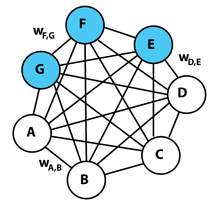
\includegraphics[width=0.5\textwidth]{Boltzmannexample.jpg}
 \caption{The structure of generic Boltzmann machine}\label{}
 \end{figure}
In the graph above, each edge represents dependency between nodes. Because there is no layer in Boltzmann, each node is possible to be connected to all other nodes with symmetric weights($w_{ij}=w_{ji}$). There is an additional node * in the machine constantly valued 1 and connected to every node, whose weights represent the thresholds. Analogously, the weights are symmetric, $w_{*i}=w_{i*}=b_{i}=\text{thresholds}$.
\paragraph{}
We use N-dimensional binary vector $X={x_{1},\dots,x_{i},\dots,x_{N}}$ to represent a configuration of the machine and $\Omega$=\{all N dimensional binary vectors\}, $card(\Omega)=2^{N}=c$. \\
As time $t=0,1,\dots,n,\dots$,
\[X(0)\rightarrow X(1)\rightarrow\cdots X(n)\rightarrow\cdots\]
So the dynamic is a stochastic process, more specifically, a Markov chain, which means
\[P(X(n)=Z|X(n-1))=P(X(n)=Z|X(n-1),\dots,X(1),X(0))\]
\textbf{Theory:} Assume that all configurations communicate in finite number of steps, i.e. ergodic. Suppose a Markov chain:
\[X(0)\rightarrow X(1)\rightarrow\cdots X(n)\rightarrow\cdots\]
If $P(X(n)=Z|X(n-1)=y)=Q(y,z)$, where $y,z \in \Omega$, Q is the transition matrix of the Markov chain, then
\begin{enumerate}
  \item Q is a $c\times c$ matrix, where $c=card(\Omega)$, $0\leq Q(y,z)\leq 1$
  \item $\sum\limits_{z\in\Omega}Q(y,z)=1$
  \item for ergodic Markov chains, $P(X(n)=Z)\rightarrow\mu(Z), n\rightarrow\infty$, X(n) keeps jumping, $\mu$=stationary distribution of the Markov chain, $0\leq\mu\leq1$ and $\sum\limits_{Z}\mu(Z)=1$
\end{enumerate}
The vector $\mu$ is computed by solving the linear system of c equations
\[\mu Q=\mu\]
yet usually hard for Boltzmann machine because c is too big.

\subsection{Origin}
\paragraph{}
The Boltzmann dynamics are derived from the Gibbs-Boltzmann distribution. We introduce the energy of current configuration $\textbf{X}$ is \[F(x)=\sum\limits_{i}b_{i}x_{i}+\sum\limits_{i,j,i\neq j}w_{ij}x_{i}x_{j}\]
The probability of $\textbf{X}=x$ is \[P(\textbf{X}=x)=\frac{exp(-F(x))}{Z}\]
where \[Z=\sum\limits_{x\in\Omega}exp(-F(x))=\text{constant}\]
We call Z is a partition function.

\subsection{Dynamics}
\paragraph{}
The symmetric weight matrix $W=(w_{ij})$ governs the dynamics, which means when $n\to \infty$, the limit probability distribution of  states will stabilize as follows:
\[P(X_i(n)=1)\to L_i(1)\]
\[P(X_i(n)=1,X_j(n)=0)\to L_{i,j}(1,0)\]
\paragraph{}
Suppose in a classification task, after 5000 iterations, the machine has stabilized. By observing the output e.g.:

\begin{table}[!hbp]\centering
\begin{tabular}{|c|c|c|c|c|c|c|}
\hline
order& n & n+1 & n+2 & n+3 & $\cdots$ & n+10000\\
\hline
Output1 & 1 &  0  &  1  &  1   &  $\cdots$ & 1 \\
\hline
Output2 &0 &  0  &  1  &  0   &  $\cdots$ & 1 \\
\hline
\end{tabular}
\end{table}

After learning, the W fixed under dynamics, and we can compute the empirical frequency of outputs: freq1 and freq2, thus we can assign them to class1 and class2 respectively as their probability.\\

\subsection{Updates}
\paragraph{}
Let's consider a configuration(n) of the Boltzmann Machine at time n.
$X_{(n)}\in \Omega$ is a random binary vector, we want to detail how $X_{(n)}$ changes into $X_{(n+1)}$ .
\paragraph{}
First, select an arbitrary order in nodes:\\
i=1, i=2, ..., i=k, ..., i=N\\
Then suppose we have $k$ epochs, then the nodes changes in such groups:
\[(1,2,\cdots,N)(1,2,\cdots,N)\cdots(1,2,\cdots,N)\]
corresponding to:\\
(time1, time2,$\cdots$,time N)(time N+1, time N+2,$\cdots$,time 2N)$\cdots$($\cdots$,time kN)\\
This is the order in which the nodes are allowed to ''change'' their state.

\subsection{Neighbours}
\paragraph{}
According to the property of Markov Chain:
\[P(X_i(n+1)=1|X(n))\equiv P(X_i(n+1)=1|\text{ state }X_j(n)\text{ for all nodes j $w_{ij}\neq 0$})\]
we can compute the influence of neighbours :
\[\sum_{j\neq *}w_{ij}\times x_j(n)+b_i=\textbf{v}\]
Therefore, the probability p(n):
\begin{align*}
P(X_i(n+1)=1|\text{ state of neighbours})=\frac1{1+e^{-v}}= \sigma(v)
\end{align*}
which is close to 1 when v is very large\\
and is close to 0 when v is very small low negative value.\\
\paragraph{}
Since we have got the probability of activating a node $p$, we could decide the value of the node with Bernoulli(p, 1-p): Firstly, generate a uniformly distributed random number between 0 and 1, if this number is between 0 and $p$, the node is activated i.e., $X_{i}(n+1)=1$, otherwise, it is not.
\subsection{Learning Algorithm}
The learning of generic Boltzmann machines is achieved by computing the average coactivity for arbitrary pairs of connected nodes.\\
\textbf{Definition:} Suppose i and j are two arbitrary nodes, K is the number of epochs,
\[CoAct(i,j)=\frac{1}{K}\sum\limits_{n=1}^{KN}x_{i}(n)x_{j}(n)\]
We run twice for each input and compute their different coactivities each time. The first one is called the unclamped coactivity, i.e., the frequency of simultaneous activity between i and j \[x_{i}=1,\ x_{j}=1\]
The second one is called the clamped coactivity. We clamp the output nodes and implement the update procedure of the other nodes, then compute the coactivities.\\
The goal is to maximize the probability
\[P(OUT=correct|IN)\]
We use gradient ascent to optimize it with respect to weights(biases included).\\
After each training batch, the update of weights:
\[\Delta w_{ij}=\epsilon [CoAct(i,j)_{clamped}-CoAct(i,j)_{unclamped}]\]
\subsection{Performance}
After completing the training, we present all inputs into it to evaluate the performance of the machine. Fix all the weights and keep outputs unclamped first, then compute how often correct answer occurs in the classification of outputs. Same examination could be done to evaluate the performance on test set.
\clearpage
\section{Restricted Boltzmann Machine}
\subsection{Introduction}
Although, they could be used for classification tasks, the primary goal of restricted Boltzmann machines is to build more efficient auto-encoders.
\begin{figure}[H]
 \centering
%  % Requires \usepackage{graphicx}
 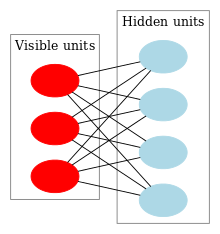
\includegraphics[width=0.5\textwidth]{Restricted_Boltzmann_machine.jpg}
 \caption{The structure of restricted Boltzmann machine}\label{}
 \end{figure}
As we can see from the structure, there are layer structures but no connection between nodes in the same layer. The connections between different layers are symmetric as in generic ones:
\[w_{ij}=w_{ji}\]
The nature of nodes is the same as generic ones, binary. There is an additional node * constantly valued 1 representing the threshold. It is connected to all nodes in both hidden and visible layers. Besides, the automatic learning follows the same rule as generic ones, yet computation is faster. More specifically, in a three-layer restricted Boltzmann machine, the number of nodes in the visible layer is the same as the input layer for auto-encoders. That is:
\[n(V)=n(Input\ nodes)\]
And the goal is to achieve:
\[OUTPUT\simeq INPUT\]
In classification tasks, the number of nodes in the visible layer is the number of classes. That is:
\[n(V)=\# \ classes\]
\subsection{Update}
\paragraph{}
With one case input, to update the whole hidden layer, we fix the nodes in visible layer $V$, and fix the Input layer. Take $h_j$ in hidden layer for instance, we calculate the influence of neighbours :
\begin{align*}
v_j&=w_{j*}\cdot1+\sum\limits_{i\in V}w_{ji}v_i+\sum_{k\in \text{INPUT}}u_{jk}\cdot IN_k\\
&=b_j+\sum\limits_{i}w_{ji}v_i+\sum_{k}u_{jk}\cdot IN_k
\end{align*}
Then, we can compute the probability:
\[P_j=\sigma(v_j)=\frac1 {1+e^{-v_j}}\]
To update the value for node $h_j$, we generate a random number R $\sim$ uniform distribution Unif[0,1]. \\
\[\hat{h_j}=1\text{, if R}\leq P\]
\[\hat{h_j}=0\text{, if R}\geq P\]
\paragraph{}
Similarly, to update the whole visible layer, we fix the nodes in hidden layer $H$.\\
Take $v_i$ in visible layer for instance, we calculate the influence of its neighbours :
\[v_i=b_i+\sum_j w_{ij}\hat {h_j}\]
Then compute the probability:
\[p_i=\sigma(v_i)=\frac1{1+e^{-v_i}}\]
By generating a random number $r$ $\sim$ Unif[0,1]:
\[\hat{v_i}=1\text{, if r}\leq p_i\]
\[\hat{v_i}=0\text{, if r}\geq p_i\]
Now we have updated the whole configuration of the machine, and generally we only need one update each time (Hinton 2010) even though we can do this kind of update repeatedly for getting $\hat{\hat{h}}$ and $\hat{\hat{v}}$.
\subsection{Learning Algorithm}
\paragraph{}
The learning of restricted Boltzmann machines is similar to GBM(generic Boltzmann Machine). By computing the average coactivity for arbitrary pairs of connected nodesand using Steepest Ascent or Gradient Ascent.\\
Keep small number of updates, and for $i\in V$, $j\in H$, we compute $c_{ij}$, the coactivity between node i and node j:
\[c_{ij}=v_i\times h_j\text{ for one Input}\]
Then the mini batch is chosen between 10-100 cases, e.g. 50 cases per batch.\\
Then the Coactivity is:
\[CoAct=\frac1{50}\sum_{50\ cases}v_i\times h_j\]
representing each pair in the CoActivity Matrix for one mini batch size of 50 cases.

We run twice for each input and compute their different coactivities each time. The first one is called the unclamped coactivity, i.e., the frequency of simultaneous activity between i and j \[x_{i}=1,\ x_{j}=1\]
The second one is called the clamped coactivity. We fix correct answer in the visible layer and only update nodes in the hidden layer $\hat{h}$, then compute the coactivities:
\[c(i,j)_{clamped}=\frac1{50}\sum_{50\ cases}v_i\times\hat{h_j}\]
And now we have the clamped coactivity matrix:
\[c(i,j)_{clamped}\to c(i,j)_{data}\]

We use gradient ascent to optimize it with respect to weights(biases included).\\
After each training batch, the update of weights:
\[\Delta w_{ij}=\epsilon \times[CoAct(i,j)_{clamped}-CoAct(i,j)_{unclamped}]\]

\paragraph{}
It is worth mentioned that during learning, for the goal of fast run, we only need to run small number of epochs, e.g., 1 or 2 epochs.

\subsection{Monitoring Performance}
\paragraph{}
To check if the learning is going well, we monitor the percentage error on the visible layer which we can observe easily.\\
After each epoch, run the whole training set on the machine case by case. Then, take classification task for example, we compute the frequency of all output layer nodes for one particular class and decide the target class by choosing the class corresponding to the largest frequency value. Thus, we can compute the correct number of outputs with respect to the true classification and evaluate the performance of learning.
\clearpage
\section{Hinton's Paper}
\subsection{Introduction}
\paragraph{}
Hinton's guide to training restricted Boltzmann machines is based on auto-encoder, yet there is a section showing how to do discrimination with restricted Boltamann machines(Sec.16). We first present the structure of restricted Boltzmann machine for auto-encoders.
\paragraph{}There are only two layers in a restricted Boltzmann machine for auto-encoder, visible layer $V$ and hidden layer $H$. Intuitively, the visible layer $V$ is both input and output layer since the original and reconstructed data  are both in it. Generally, we input cases to the visible layer, then update the hidden layer with the original data, then update the visible layer with the hidden layer reversely to obtain the reconstructed data. Thus there is no need of a third layer.
\subsection{Update}
\paragraph{}A joint configuration (V,H) has an energy:
\[E(V,H)=-\sum\limits_i a_i v_i-\sum\limits_jb_j h_j-\sum\limits_{i,j}w_{ij}v_i h_j\]
where $a_i$ and $b_j$ are the biases of visible and hidden layer, $w_{ij}$ are the weights between them. The probability to each possible pair of visible and hidden layer is given by:
\[P(V,H)=\frac1Ze^{-E(V,H)}\]
where \[Z=\sum\limits_{V,H}e^{-E(V,H)}\]
A very simple learning rule for performing the steepest gradient ascent is given by:
\[\Delta w_{ij}=\epsilon (\langle v_i,h_j\rangle_{data}-\langle v_i,h_j\rangle_{model})\]
where $\epsilon$ is a learning rate and the angle brackets are used to denote expectations under the distribution specified above.
\paragraph{}Given a random training case V, the binary state $h_j$ is activated i.e., valued 1 with probability:
\[P(h_j=1|V)=\sigma(b_j+\sum\limits_iw_{ij}v_i)\]
where $\sigma$ is the sigmoid function
\[\sigma(x)=\frac1{1+e^{-x}}\]
Then we could get an unbiased sample of $\langle v_i,h_j\rangle_{data}$ easily.
\paragraph{}
Analogously, we could update the visible layer node $v_i$ given the hidden layer with activation probability:
\[P(v_i=1|H)=\sigma(a_i+\sum\limits_jw_{ji}h_j)\]
where $w_{ij}=w_{ji}$.
To get an unbiased sample of $\langle v_i,h_j\rangle_{model}$, we need to reconstruct the visible layer with the equation above and compute $v_ih_j$, where $v_i$ is the reconstructed visible node value. The change of weights is then
\[\Delta w_{ij}=\epsilon (\langle v_i,h_j\rangle_{data}-\langle v_i,h_j\rangle_{recon})\]
\subsection{Mini-batch}
To improve the performance of training, we divide the training set into mini-batches. When computing the stochastic gradient under mini-batch, we assume that they multiply the average gradient computed on a mini-batch, not the total gradient on a mini-batch. Too large mini-batch size could be a serious mistake.
\paragraph{}For classification task with small number of equiprobable classes, it is ideal to use a mini-batch with size of the number of classes and each mini-batch should contain one example of each class. For other datasets, use the mini-batch size about 10.
\subsection{Overfitting}
\paragraph{}One simple way to avoid overfitting is to stop learning when the probability of obtaining correct datapoint starts to decrease for held out validation set. A recipe for it is that compute the average free energy of a representative subset of the training data and compare it with the average energy of a validation set.
\subsection{Learning Rate}
\paragraph{}If the learning rate is much too large, the reconstruction error usually increases dramatically and the weights may explode. However, if the learning rate is reduced while the network is learning normally, the reconstruction error will usually fall significantly and it is generally accompanied by slower learning in the long term. The recipe for it is to look at the histogram of the weight updates and a histogram of the weights. The updates should be $10^{-3}$ times the weights(to within about an order of magnitude).
\subsection{Initialization of Weights}
\paragraph{}The weights are typically initialized to small random values chosen from a zero-mean Gaussian with a standard deviation of about 0.01, $N(0,0.0001)$. It is usually helpful to initialize the bias of visible unit i to
\[log\frac{p_i}{1-p_i}\]
where $p_i$ is the proportion of training vectors in which unit i is on. Look at the activities of the hidden units occasionally to check that they are not always on or off.
\subsection{RBM for Discrimination}
\paragraph{}
According to Hinton, there are three obvious ways of using RBM's for discriminations. The first way is to use the hidden features learned by RBM as the inputs for some standard discriminative method. The second method is to train a separate RBM on each class. The third method is to train a joint density model using a single RBM that has two sets of visible units.\\
Here we discuss the second and the third way.\\
\subsubsection{The second way and the computation of the free energy of a visible vector}
\paragraph{}
The free energy of visible \textbf{v} is the energy that a single configuration would need to have in order to have the same probability as all of the configuration that contain \textbf{v}:
\[e^{-F(v)}=\sum_{\textbf{h}}e^{-E(v,h)}\]
It is also given by the expected energy minus the entropy:
\[F(\textbf{v})=-\sum_iv_ia_i-\sum_jp_jx_j+\sum_j[p_j\ \text{log }p_j+(1-p_j)\text{ log }(1-p_j)]\]
where $x_j=b_j+\sum\limits_iv_iw_{ij}$ is the total input to hidden unit j and $p_j=\sigma(x_j)$ is the probability that $h_j=1$ given \textbf{v}. A good way to compute F(\textbf{v}) is to use yet another expression for the free energy:
\[F(\textbf{v})=-\sum_iv_ia_i-\sum_j\text{ log }(1+e^{x_j})\]
\paragraph{}
After training, the free energy of a test vector \textbf{t} is computed for each class-specific RBM. The log probability that the RBM trained on class c assigns to the test vector is given by:
\[\text{ log }p(\textbf{t}|c)=-F_c(\textbf{t})-\text{log }Z_c\]
where $Z_c$ is the partition function of that RBM.\\
If the number of classes is small it is easy to deal with unknown log partition functions by simply training a "softmax" model (on a separate training set) to predict the class from the free energies of all of the class specific RBMs:
\[\text{log }p(\text{class} =c|\textbf{t})=\frac{e^{-F_c(\textbf{t})-\text{log }\hat{Z_c}}}{\sum\limits_de^{-F_d(\textbf{t})-\text{log }\hat{Z_d}}}\]
where the $\hat{Z}$ are parameters that are learned by maximum likelihood training of the softmax.
\subsubsection{The third way}
\paragraph{}
In addition to the units that represent a data vector, there is a "softmax" label unit that represents the class. After training, each possible label is tried in turn with a test vector and the one that gives the lowest free energy is chosen as the most likely class. Again, it is possible to combine discriminative and generative training of the joint the joint RBM by using discriminative gradients that are the derivatives of the log probability of the correct class(Hinton 2007):
\[\text{log }p(\text{class }=c|\textbf{t})=\frac{e^{-F_c(\textbf{t})}}{\sum_d\limits e^{-F_d(\textbf{t})}}\]


\clearpage
\section{Implementation of RBM}
\subsection{Description of Dataset}
\paragraph{}We select intra-day prices of 757 stocks with a frequency of 60 seconds which includes 5000 cases. Since the original data is continuous and numerical, we need to binarize it to input it into a Boltzmann machine. We first compute the moving average of 10 previous cases. Then the data $X_i$ is 1 if
\[X_i\geq \frac 1{10}\sum_{j=1}^{10}X_{i-j}\]
otherwise, $X_i=0$. Then the dimension of binarized input and output are both 757 and 5000 cases in total.
\subsection{Implementation of RBM Auto-encoders}
\paragraph{}We use matlab to implement a restricted Boltzmann machine for auto-encoder. Since there is no existing package for RBM in matlab, we construct the machine by ourselves. We first initialize the layers as null vectors, weights matrix as standard normal distributed random numbers, biases as zero vectors and learning rate $\epsilon$ as 0.1. It is worth mentioned that we tie the weights between hidden layer and output layer and those between input layer and hidden layer, this structure is equivalent to it in Hinton's paper. Then we randomly permuted the data set and divide it into batches with size of 100 and repeat this manipulation at the beginning of each epoch. We choose sigmoid as the response function. During training, we first compute the clamped coactivity between hidden layer and output layer.
\begin{lstlisting}[language=Matlab]
  poshidprobs = 1./(1 + exp(-data*vishid - repmat(hidbiases,batchsize,1)));
  posprods    = data' * poshidprobs;
\end{lstlisting}
where data is the matrix of input in one batch, poshidprobs is the activating probability matrix of the hidden layer. Then the varibale posprods is coactivity matrix with respect to each pair of hidden and output units over the whole batch. Then we update the hidden layer with the probability above.
\begin{lstlisting}[language=Matlab]
poshidstates = poshidprobs > rand(batchsize,numhid);
\end{lstlisting}
\paragraph{}
Analogously, we compute the unclamped coactivity after updating the output layer.
\begin{lstlisting}[language=Matlab]
  negdata = 1./(1 + exp(-poshidstates*vishid' - repmat(visbiases,batchsize,1)));
  neghidprobs = 1./(1 + exp(-negdata*vishid - repmat(hidbiases,batchsize,1)));
  negprods  = negdata'*neghidprobs;
\end{lstlisting}
Then we could update the weights(biases included) with the coactivities computed above.
\begin{lstlisting}[language=Matlab]
    vishidinc = epsilonw*( (posprods-negprods)/batchsize);
\end{lstlisting}
As the code has shown, we compute the difference of clamped and unclamped coactivities and multiply it with the learning rate $\epsilon$ and average over batch. Then this variable is the increment of weights.
\paragraph{}
The training with sparsity could be achieved in matlab by adding a penalty term consisting of the cross entropy between the empirical sparsity of hidden layer and the preset sparsity level into the increment of weights.
\paragraph{}
We tested several sizes for the hidden layer $h$. We initially tried with 105, which is the result of the eigenvalue ratio with respect to significance level of 90\% PCA analysis. However, compared with 60, 75, 91, 105, 120 we decided most suitable hidden layer size is 91. Furthermore, we tested the different initialization parameters regarding the Normal distribution $N(0,0.0001)$, $N(0,0.0025)$ and $N(0,0.01)$, and we found that the best initialization is standard deviation is 0.1. The most suitable learning rates we choose is constant 0.1 compared with $\frac{\text{learning rate}}n$. \\
For the batch size we choose, after comparing 100,200 and 500, we find batch size of 100 leading to 50 batches is the most suitable choice.

\paragraph{}
The current gradient norm $||G(n)||$, mean and standard deviation of we;kights is computed by :
\begin{lstlisting}[language=Matlab]
  gradient(global_step)=norm(vishidinc/epsilonw);
  meanwei(global_step)=mean(mean(vishid));
  stdevwei(global_step)=std(reshape(vishid,[1,numdims*numhid]));
\end{lstlisting}
And the evolution plots are listed as follows:
\begin{figure}[H]
 \centering
  % Requires \usepackage{graphicx}
 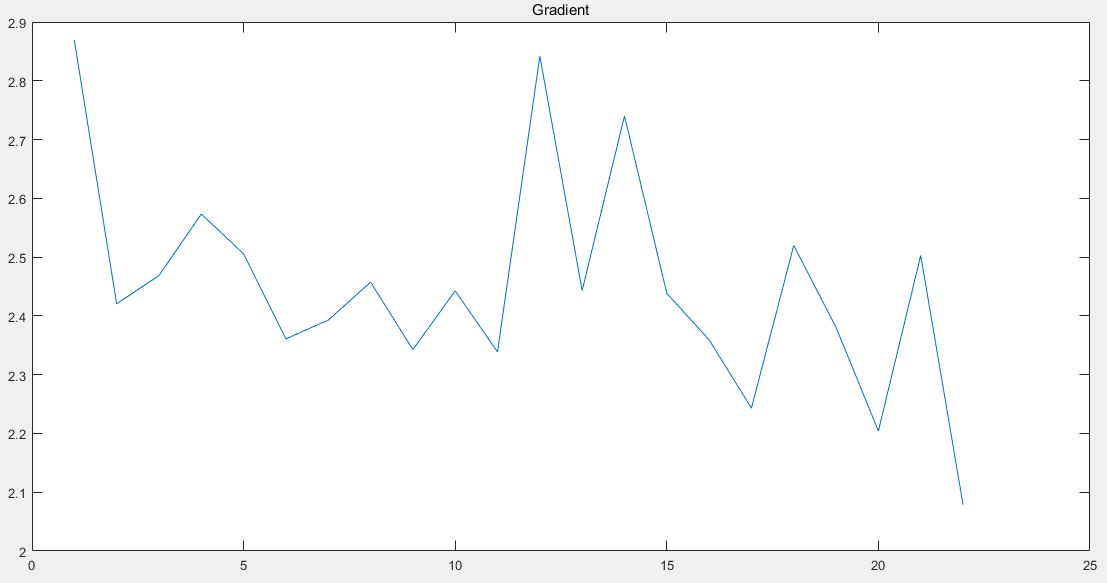
\includegraphics[width=1.2\textwidth]{Gradient}
 \caption{Gradient}\label{}
 \end{figure}
As we could see from the plot, the gradient decreases rapidly at the beginning of training and gradually get steady as the the number of iterations grows.

\begin{figure}[H]
 \centering
  % Requires \usepackage{graphicx}
 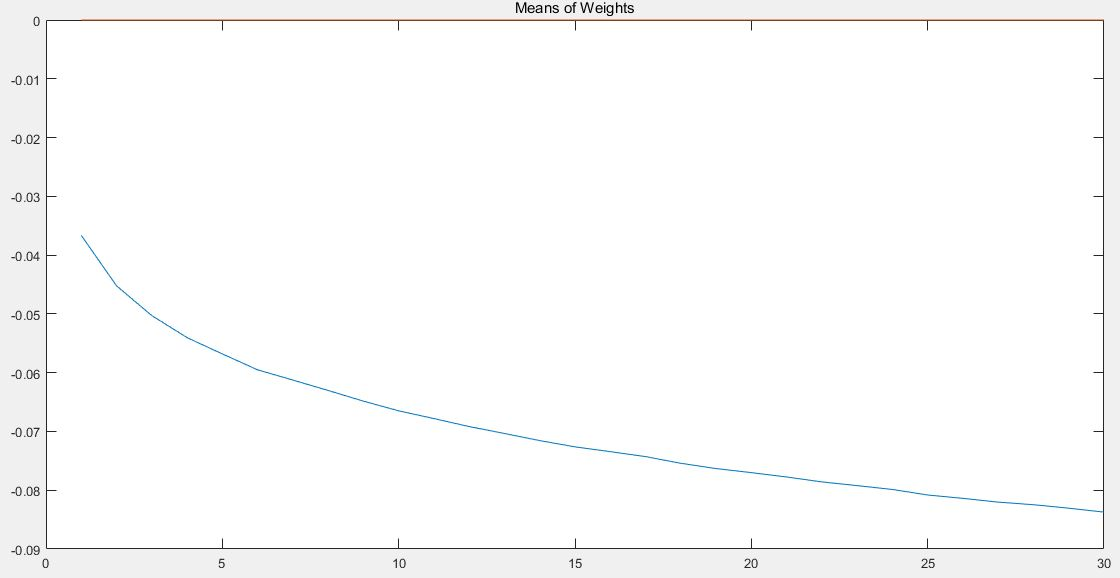
\includegraphics[width=1.2\textwidth]{MeanofWeights}
 \caption{Mean of Weights}\label{}
 \end{figure}
As the plot has shown, the mean of weights increases during training. This is the same as we expected since the initial mean is 0 and after updates of the weights, it is reasonable to make the mean away from 0.
 \begin{figure}[H]
 \centering
  % Requires \usepackage{graphicx}
 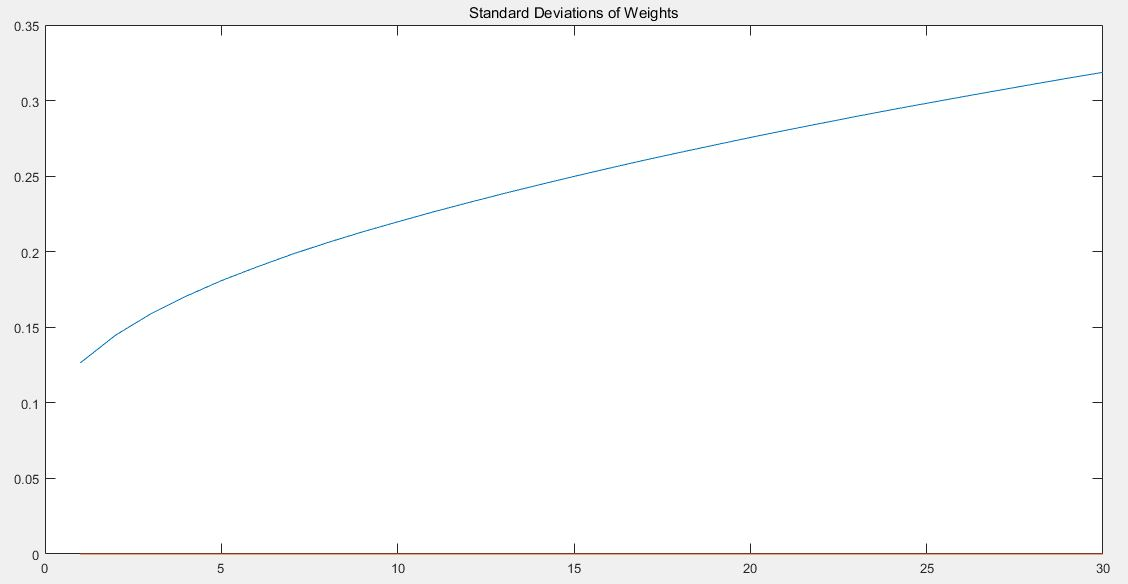
\includegraphics[width=1.2\textwidth]{StdevofWeights}
 \caption{Stdev of Weights}\label{}
 \end{figure}
Similar to the mean, the standard deviation increases during training since different weights between different pairs of nodes generally have various functions for reconstruction of inputs. So it is understandable that the standard deviation increases.
 \begin{figure}[H]
 \centering
  % Requires \usepackage{graphicx}
 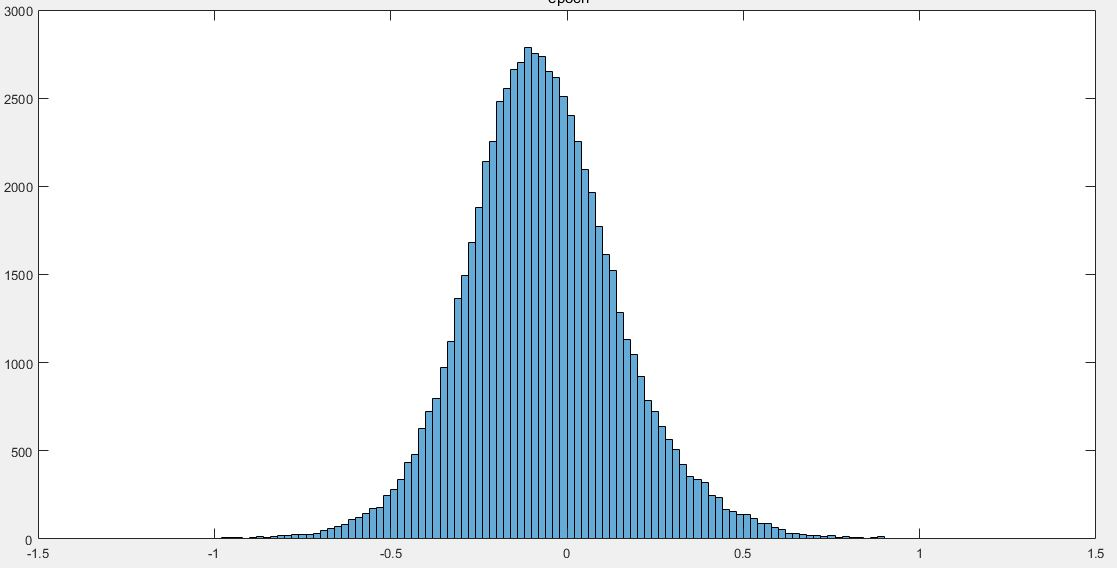
\includegraphics[width=1.2\textwidth]{hist1.jpg}
 \caption{histogram after 10 epochs}\label{}
 \end{figure}
 \begin{figure}[H]
 \centering
  % Requires \usepackage{graphicx}
 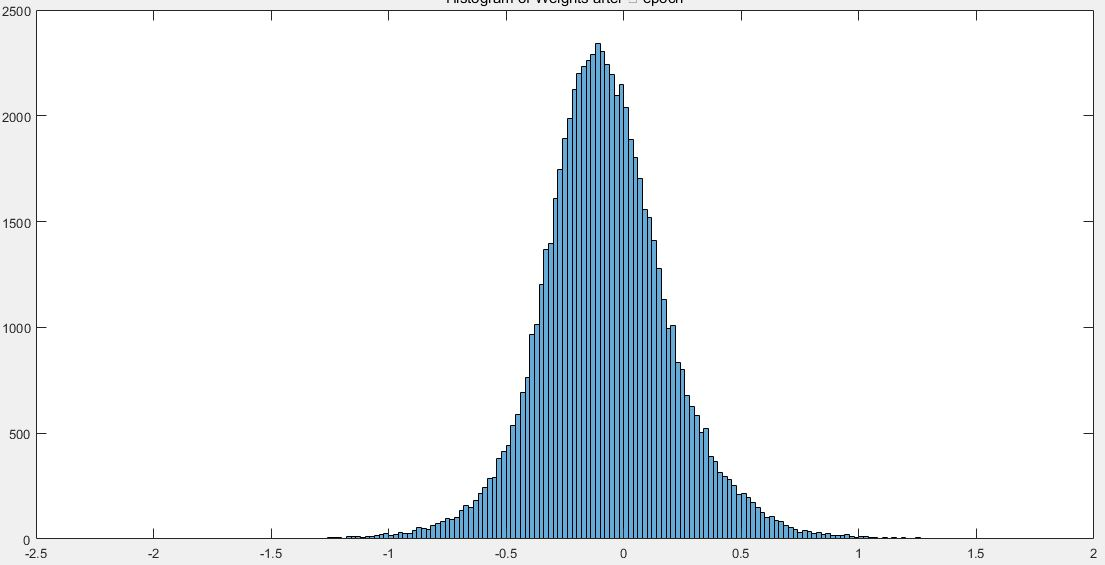
\includegraphics[width=1.2\textwidth]{hist2.jpg}
 \caption{histogram after 20 epochs}\label{}
 \end{figure}
\paragraph{}
As can be seen from the histogram, the weights are distributed between -1.5 and 1.5. We can consider it as a normal distribution with its peak at the value of approximately -0.05 and the histogram shows that nearly 2800 nodes are in this peak.

  \begin{figure}[H]
 \centering
  % Requires \usepackage{graphicx}
 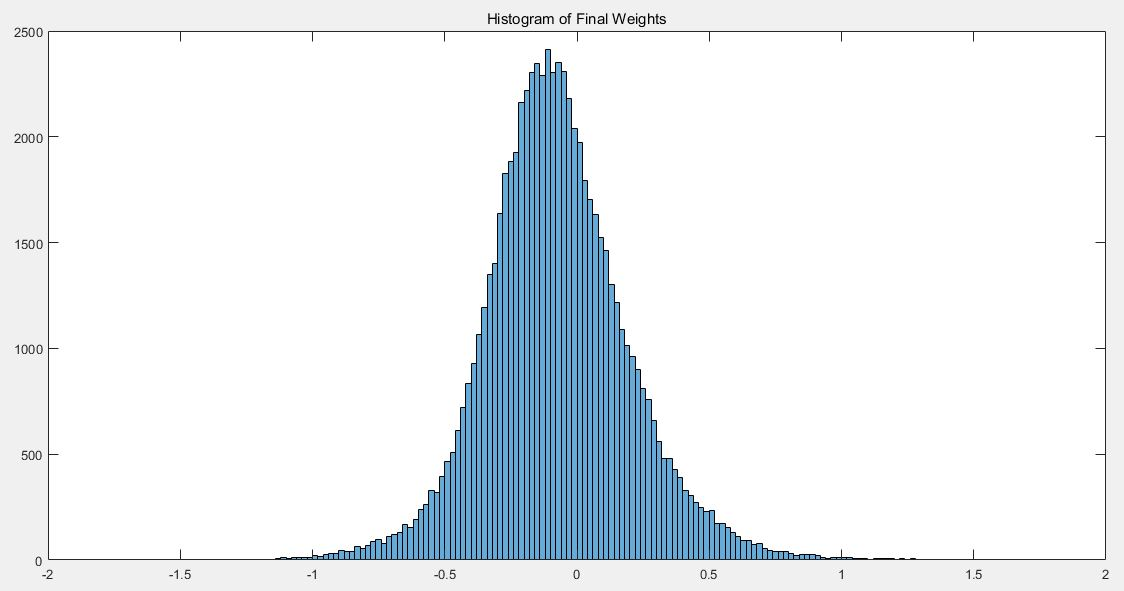
\includegraphics[width=1.2\textwidth]{Finhist}
 \caption{histogram of final epoch}\label{}
 \end{figure}
\paragraph{}
As can be seen in the plot, the histogram after final epoch becomes more flat, which means the number of nodes distributed in the peak interval is less than the histogram after 10 epochs. Also, the peak value becomes smaller, which is at around 2450 much lower than the previous peak 2800. This may be explained by the fact that with the learning process continues, the weight matrix becomes more stable and this leads to a more flat histogram.


\paragraph{}Here we decide to use the gradient as our stopping rule, after the change of gradient within two consecutive iteration is smaller than our preset tolerance(implying that the learning velocity is slower than some preset level), we terminate the learning process. For example, after epoch 22 , the gradient here is 2.079, which is smaller than our preset tolerance 2.1. So we terminate our learning process after $22*50=1100$ iterations.
\paragraph{}
\begin{lstlisting}[language=Matlab]
for n=1:numcases
    hidden=1./(1 + exp(-data(n,:)*vishid - hidbiases));
    out(n,:,1)=1./(1 + exp(-hidden*vishid' - visbiases));
    for i=1:20
        hidden=1./(1 + exp(-out(n,:,i)*vishid - hidbiases));
        out(n,:,i+1)=1./(1 + exp(-hidden*vishid' - visbiases));
    end
    aveout(n)=norm(mean(out(n,:,:),3)-data(n,:))^2/numdims;
end
MSE=mean(aveout);
\end{lstlisting}
As the above codes have shown, for each case, we first update the hidden layer with the trained weights and sigmoid function, then update the output layer with the transpose of the weight matrix and sigmoid function. After repeating this update for 20 times, we could compute the reconstruction error of any given case $X(n)$ by:
\[MSE(n)=\frac1r||y(n)-X(n)||^2\]
where r is the dimension of inputs, y(n) is the average of 20 reconstructed outputs.
\paragraph{}The best average MSE over whole data set we have is $0.1011$, which is under the hyper-parameter selection of 91 hidden units and weights' initial standard deviation of $0.1$.

\section{Appendix: Matlab Codes}
The main script:
\begin{lstlisting}[language=Matlab]

% This program trains Restricted Boltzmann Machine in which
% visible, binary, stochastic pixels are connected to
% hidden, binary, stochastic feature detectors using symmetrically
% weighted connections. Learning is done with 1-step Contrastive Divergence.
% The program assumes that the following variables are set externally:
% maxepoch  -- maximum number of epochs
% numhid    -- number of hidden units
% batchdata -- the data that is divided into batches (numcases numdims numbatches)
% restart   -- set to 1 if learning starts from beginning
clear;clc;
restart=1;
epsilonw      = 0.1;   % Learning rate for weights
epsilonvb     = 0.1;   % Learning rate for biases of visible units
epsilonhb     = 0.1;   % Learning rate for biases of hidden units
weightcost  = 0;
initialmomentum  = 0;
finalmomentum    = 0;
batchdata=makebatch('bidata.csv');
numhid=91;
maxepoch=30;

totdata=csvread('bidata.csv');
totnum=size(totdata,1);
numbatches=totnum/100;
numdims  =  size(totdata,2);
batchsize = 100;


if restart ==1
  restart=0;
  epoch=1;

% Initializing symmetric weights and biases.

  vishid     = 0.1*randn(numdims, numhid);
  hidbiases  = zeros(1,numhid);
  visbiases  = zeros(1,numdims);
  poshidprobs = zeros(batchsize,numhid);
  neghidprobs = zeros(batchsize,numhid);
  posprods    = zeros(numdims,numhid);
  negprods    = zeros(numdims,numhid);
  vishidinc  = zeros(numdims,numhid);
  hidbiasinc = zeros(1,numhid);
  visbiasinc = zeros(1,numdims);
  batchposhidprobs=zeros(batchsize,numhid,numbatches);
  global_step=1;
  gradient=zeros(maxepoch);
  meanwei=zeros(maxepoch);
  stdevwei=zeros(maxepoch);
end

for epoch = 1:maxepoch
 batchdata=zeros(batchsize, numdims, numbatches);
 rng(sum(100*clock));
 randomorder=randperm(totnum);
 for b=1:numbatches
  batchdata(:,:,b) = totdata(randomorder(1+(b-1)*batchsize:b*batchsize), :);
 end


 fprintf(1,'epoch \%d\r',epoch);
 errsum=0;
 for batch = 1:numbatches
 fprintf(1,'epoch \%d batch \%d\r',epoch,batch);

%%%%%%%%% START POSITIVE PHASE %%%%%%%%%%%%%%%%%%%%%%%%%%%%%%%%%%%%%%%%%%%%%%%%%%%
  data = batchdata(:,:,batch);
  poshidprobs = 1./(1 + exp(-data*vishid - repmat(hidbiases,batchsize,1)));
  batchposhidprobs(:,:,batch)=poshidprobs;
  posprods    = data' * poshidprobs;
  poshidact   = sum(poshidprobs);
  posvisact = sum(data);

%%%%%%%%% END OF POSITIVE PHASE  %%%%%%%%%%%%%%%%%%%%%%%%%%%%%%%%%%%%%%%%%%%%%%%%%
  poshidstates = poshidprobs > rand(batchsize,numhid);

%%%%%%%%% START NEGATIVE PHASE  %%%%%%%%%%%%%%%%%%%%%%%%%%%%%%%%%%%%%%%%%%%%%%%%%%
  negdata = 1./(1 + exp(-poshidstates*vishid' - repmat(visbiases,batchsize,1)));
  neghidprobs = 1./(1 + exp(-negdata*vishid - repmat(hidbiases,batchsize,1)));
  negprods  = negdata'*neghidprobs;
  neghidact = sum(neghidprobs);
  negvisact = sum(negdata);

%%%%%%%%% END OF NEGATIVE PHASE %%%%%%%%%%%%%%%%%%%%%%%%%%%%%%%%%%%%%%%%%%%%%%%%%%
  err= sum(sum( (data-negdata).^2 ));
  errsum = err + errsum;

   if epoch>5
     momentum=finalmomentum;
   else
     momentum=initialmomentum;
   end

%%%%%%%%% UPDATE WEIGHTS AND BIASES %%%%%%%%%%%%%%%%%%%%%%%%%%%%%%%%%%%%%%%%%%%%%%%
    vishidinc = epsilonw*( (posprods-negprods)/batchsize);
    visbiasinc = momentum*visbiasinc + (epsilonvb/batchsize)*(posvisact-negvisact);
    hidbiasinc = momentum*hidbiasinc + (epsilonhb/batchsize)*(poshidact-neghidact);

    vishid = vishid + vishidinc;
    visbiases = visbiases + visbiasinc;
    hidbiases = hidbiases + hidbiasinc;

%%%%%%%%%%%%%%%% END OF UPDATES %%%%%%%%%%%%%%%%%%%%%%%%%%%%%%%%%%%%%%%%%%%%%%%%%%%%
  gradient(epoch)=norm(vishidinc/epsilonw);
  meanwei(epoch)=mean(mean(vishid));
  stdevwei(epoch)=std(reshape(vishid,[1,numdims*numhid]));
  global_step=global_step+1;
 end

 if rem(epoch,10)==0
  figure
  histogram(vishid);
  title(['Histogram of Weights after ' epoch ' epoch']);
 end

  fprintf(1, 'epoch \%4i error \%6.1f  \n', epoch, err);
  if gradient(epoch)<2.1
      break
  end
end
figure
plot(1:maxepoch, gradient)
title('Gradient')
figure
plot(1:maxepoch, meanwei)
title('Means of Weights')
figure
plot(1:maxepoch, stdevwei)
title('Standard Deviations of Weights')
figure
histogram(vishid);
title('Histogram of Final Weights');

data=csvread('bidata.csv');
numcases=size(data,1);
out=zeros(numcases,numdims,21);
aveout=zeros(numcases);
for n=1:numcases
    hidden=1./(1 + exp(-data(n,:)*vishid - hidbiases));
    out(n,:,1)=1./(1 + exp(-hidden*vishid' - visbiases));
    for i=1:20
        hidden=1./(1 + exp(-out(n,:,i)*vishid - hidbiases));
        out(n,:,i+1)=1./(1 + exp(-hidden*vishid' - visbiases));
    end
    aveout(n)=norm(mean(out(n,:,:),3)-data(n,:))^2/numdims;
end
aveout=aveout(:,1);
MSE=mean(aveout);
\end{lstlisting}

The function for making batches:
\begin{lstlisting}[language=Matlab]
function batchdata=makebatch(filename)
data=csvread(filename);
totnum=size(data,1);
fprintf(1, 'Size of the test dataset= \%5d \n', totnum);

rng(sum(100*clock)); %so we know the permutation of the training data
randomorder=randperm(totnum);

numbatches=totnum/100;
numdims  =  size(data,2);
batchsize = 100;
batchdata1 = zeros(batchsize, numdims, numbatches);

for b=1:numbatches
  batchdata1(:,:,b) = data(randomorder(1+(b-1)*batchsize:b*batchsize), :);
end
batchdata=batchdata1;
end
\end{lstlisting}
 \end{document}
